\section{Laboratory work implementation}

\subsection{Tasks and Points}

\begin{itemize}

	
	\item Advanced Level (nota 9 || 10):
	\begin{itemize}
		\item Lucreaza la proiect in echipa de 2 persoane
		\item Divizeaza task-urile si descrie-le in raport, indicind pentru fiecare cine este responsabil pentru el.
		\item Inainte de a trece la dezvoltarea proiectului, creeaza o schema cit mai apropiata de rezultatul final (schema trebuie sa fie primul commit)
		\item Fiecare din membrii echipei va lucra pe propriul branch in git, iar una din persoane va avea grija sa faca merge cu master.
		\item Proiectul se poate afla doar in repozitoriul unui membru al echipei.
		\item Fiecare din membru va avea propriul raport care va include propriile observatii si concluzii.
		\item 	Dezvoltarea unei aplicatii: Game development (web, mobile, desktop)
\end{itemize}
\end{itemize}

\subsection{Analiza lucrarii de laborator}

Repository link: https://github.com/DanielUrsachi/duonew.git. 
\newline 
Pentru inceput, am decis particularitatile partii functionale a jocului si tipul in care va arata acesta. Am decis sa folosim un PauseMenu pentru prima lansare a aplicatiei, in cazul tastarii PuseButton si la GameOver in diferite moduri.
Am efectuat un machet pentru a defini principiile de baza a functionalului si designe-ului:
\begin{center}
\includegraphics[width=0.7\linewidth]{../duonew/AppTemplate}
\end{center}

Dupa care am Creat un repositoriu nou pe git si atasindu-l de un file aparte:
\begin{center}
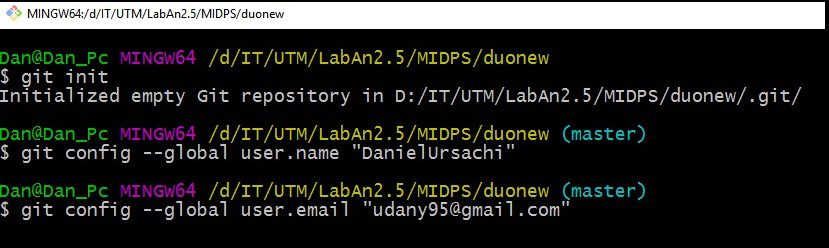
\includegraphics[width=0.7\linewidth]{screenshot001}
\end{center}

Colegul meu, Ion a adaugat acest repositoriu in acountul sau, dupa care a creat un branch nou, astfel dupa fiecare incarcare a file-urilor altuia avem nevoie de pull --rebase al celuilalt acount:
\begin{center}
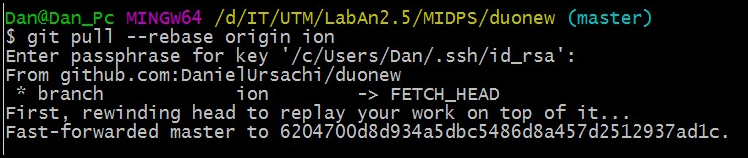
\includegraphics[width=0.7\linewidth]{screenshot002}
\end{center}

Dupa setarea corecta a git-ului, am creeat un proiect prin LibGdx care include in sine un FrameWork cu resurse, pentru gameDevelop
\begin{center}
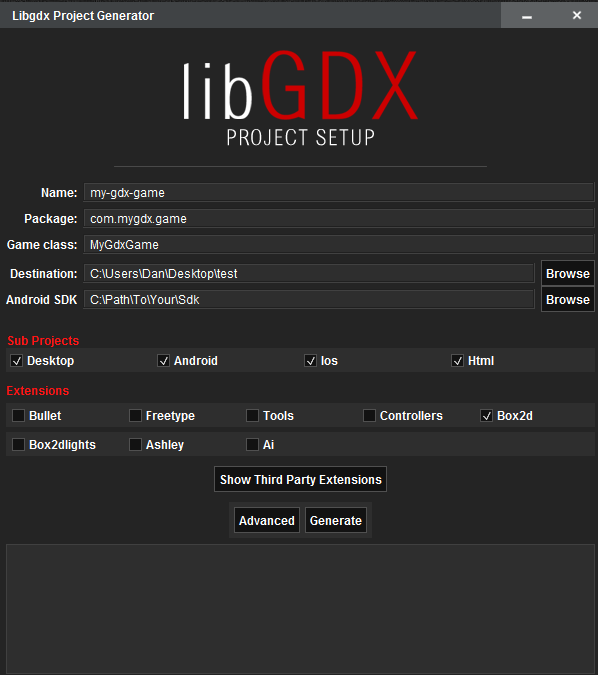
\includegraphics[width=0.7\linewidth]{screenshot003}
\end{center}

Am lansat acest proect prin AndroidStudio si am incercat compilarea Desktop si cea prin Emulator si USB Device.
Am setat lansarea Desktop si cea Android:
\begin{center}
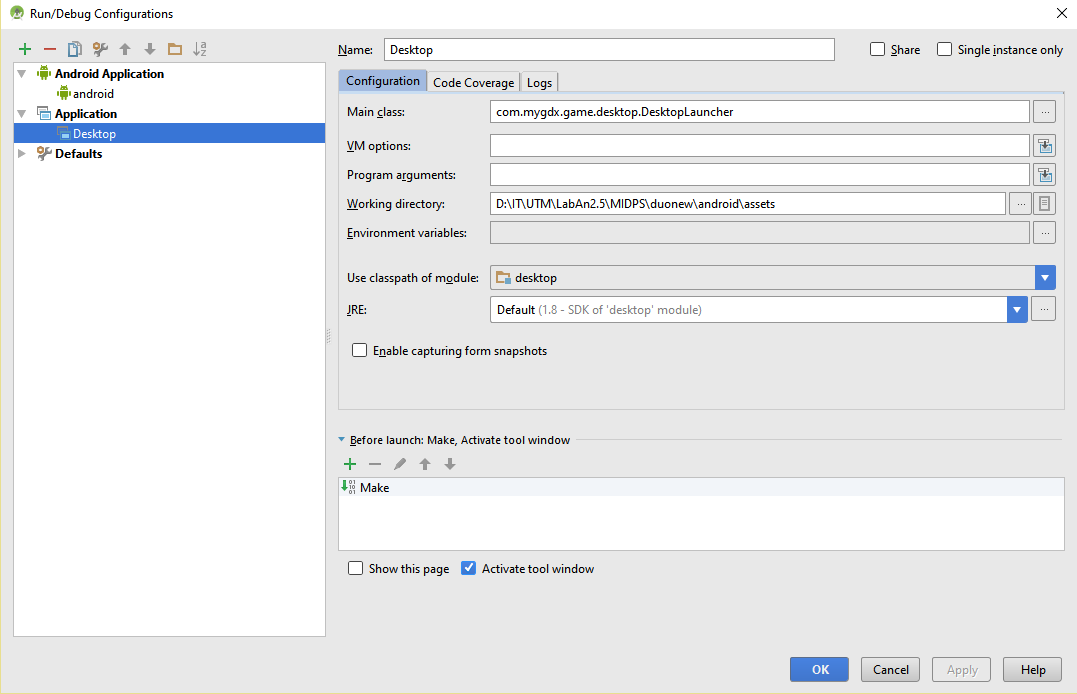
\includegraphics[width=0.7\linewidth]{screenshot004}
\end{center}
\newline 
Ion commit: a setat file-urile Launcher pentru toate platformele + adaugarea Icon
\newline \newline 
My commit: am scris in cod instrumentele de baza pentru afisarea aplicatiei, am introdus la fel Textures pentru obiectele necesare cu resurse png si am definit citeva rectangle pentru lucrul cu dimensiunea acestora. La fel am schimbat tipul de MainClass in extends Application listener pentru obtinerea overwrite methods pentru pause, resume, metode care le vom folosi pentru PauseMenu. Am instalat parametrii initiali ai celor 2 instrumente pentru jucatori in dependenta de marimile ecranului.
\begin{center}
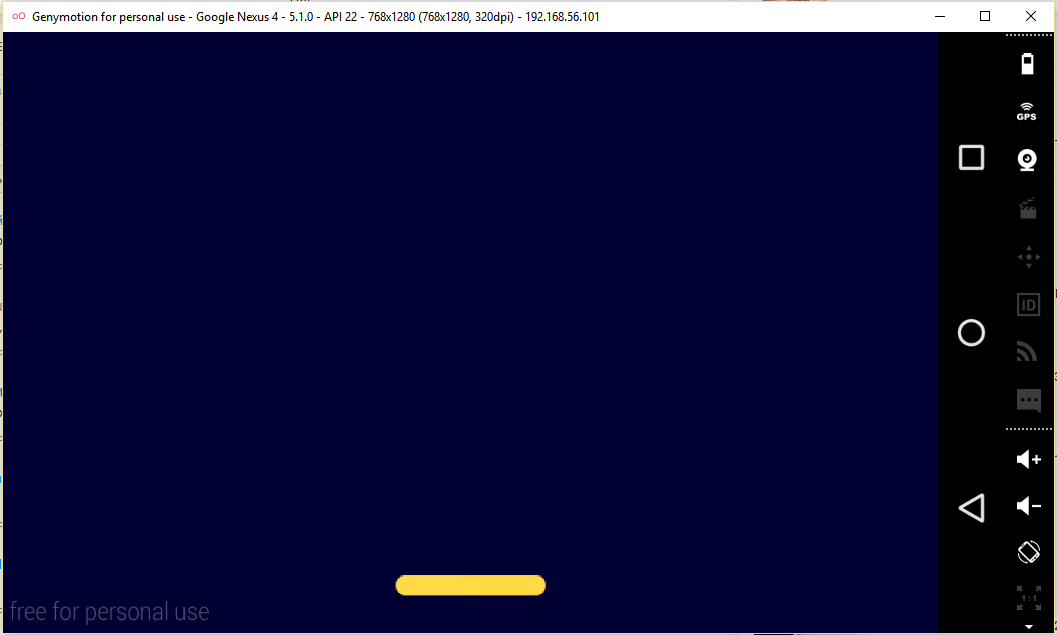
\includegraphics[width=0.7\linewidth]{screenshot005}
\end{center}

\newline \newline 
Ion commit: Implementarea PauseButton pentru ecranul activ si apelarea sa la onPause
\newline \newline
My commit: Importarea resurselor de baza png si fonturilor pentru a evita scadearea calitatii imaginii in momentul display-ului textului cu score, in cazul in care folosim scale la text. Introducerea resurselor sound, initializarea lor si introducerea in program ca Music si Sound pentru muzica continua si pentru cea de efecte. Am introdus Controlul prin Keyboard pentru versiunea web si cea desktop prin sageti tinind cont de PauseMenu. Am setat un contor de baza a score-ului si am introdus o metoda pentru desenarea obiectelor ce cad: Bomb, prin setarea unui Array de Rectangle, importarea unui iterator si afisarea acesotra in dependenta de viteza, periodicitate si actiunea pentru overlap dintre acestea si obiectele noastre. Setarea scorului ++ la fiecare render al ecranului.
\begin{center}
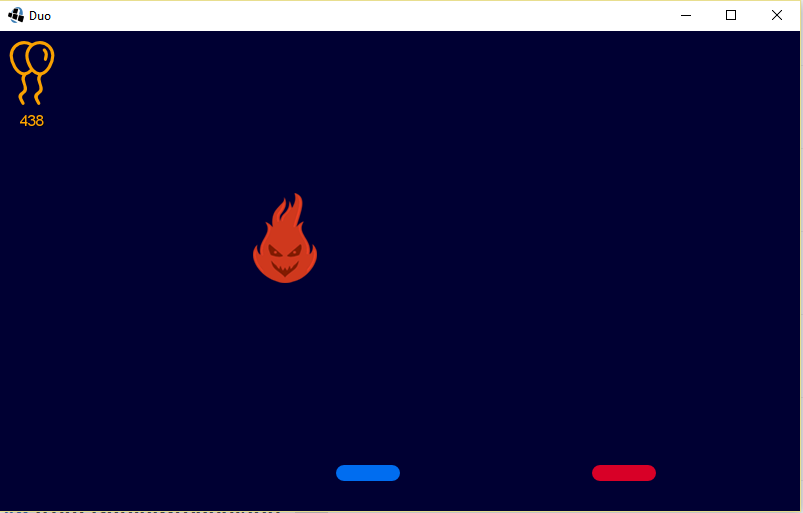
\includegraphics[width=0.7\linewidth]{screenshot006}
\end{center}

\newline \newline
Ion commit:Adaugare resurse png pentru Texturi 

\newline \newline
Ion commit:Implementarea PauseMenu

\newline \newline
My commit:Implementarea Controlului aplicatiei prin touch, ecranul reactionind la 2 degete, 2 Gdx.input.isTouched, am inlaturat bug-ul setarii pozitiei fixe a unui element atita timp cit alul se misca, am inlaturat problema a maririi vitezei daca ambele touch-uri sunt pe aceeasi parte a ecranului prin ignorare a repetarea partii ecranului de touch. Introducerea noului Icon Creeat de noi, modificarea logicii codului. Optimizarea PauseMenu, adaugarea Textures pentru acesta.
\begin{center}
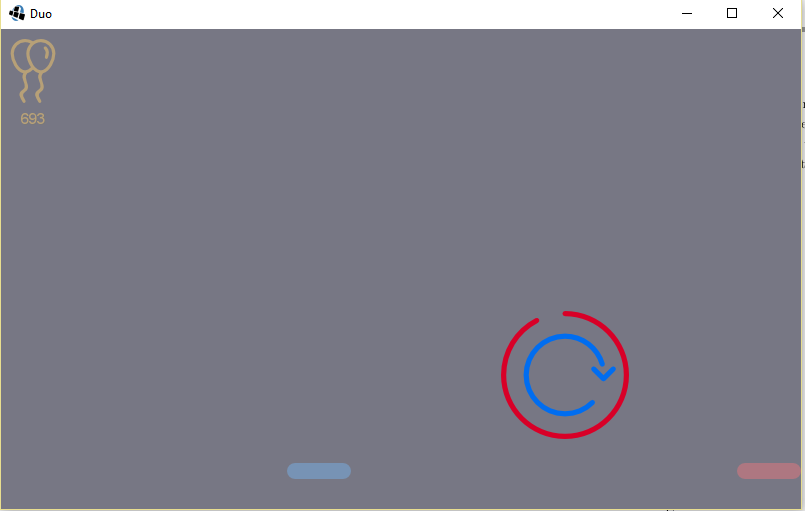
\includegraphics[width=0.7\linewidth]{screenshot007}
\end{center}

\newline \newline
Ion commit:Implemenatere BonusDrop

\newline \newline
My Commit: Rearanjarea codului, adaugarea comentariilor pentru variabile si metode, Buildul pe HTML prin comand line folosind GWT
\begin{center}
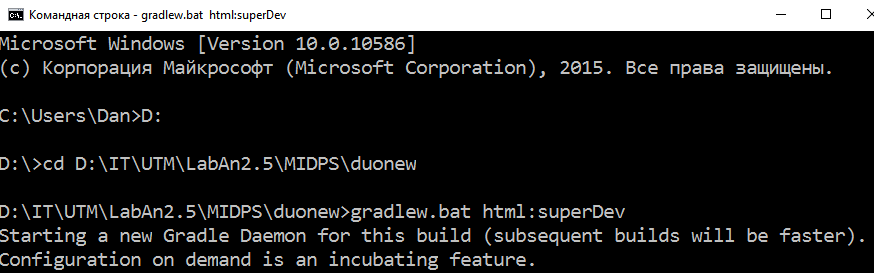
\includegraphics[width=0.7\linewidth]{screenshot008}
\end{center}
Crearea unui server virtual pe localHost pentru compilarea javascript dupa convertirea acestuia din java:
\begin{center}
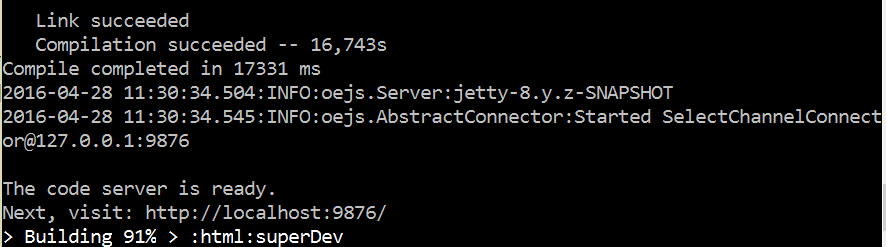
\includegraphics[width=0.7\linewidth]{screenshot009}
\end{center}
Afisarea in Browser:
\begin{center}
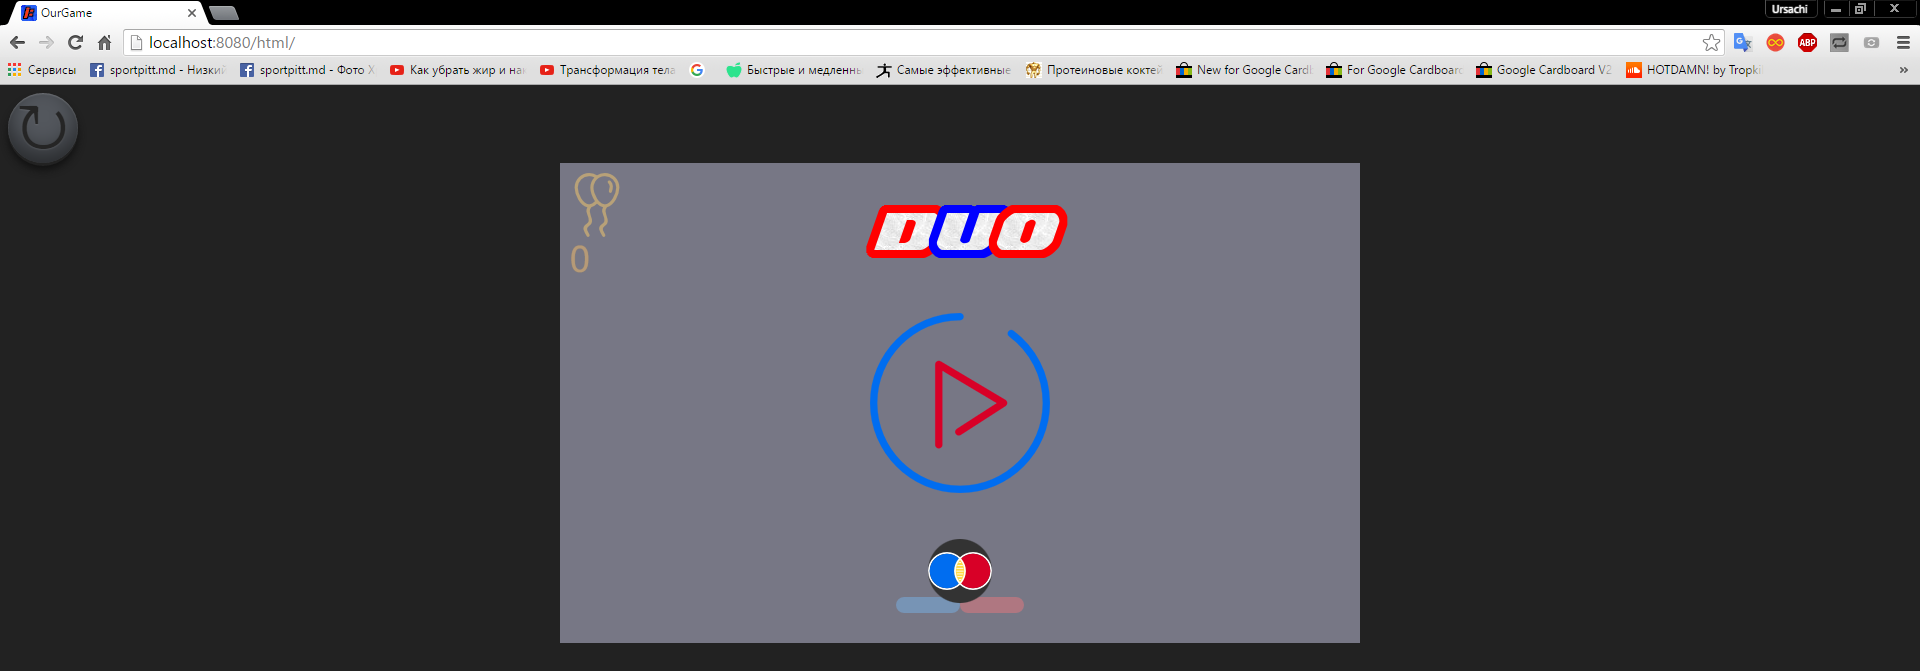
\includegraphics[width=0.7\linewidth]{screenshot010}
\end{center}

\newline \newline
MenuPause initial la primul launch Aplication
\begin{center}
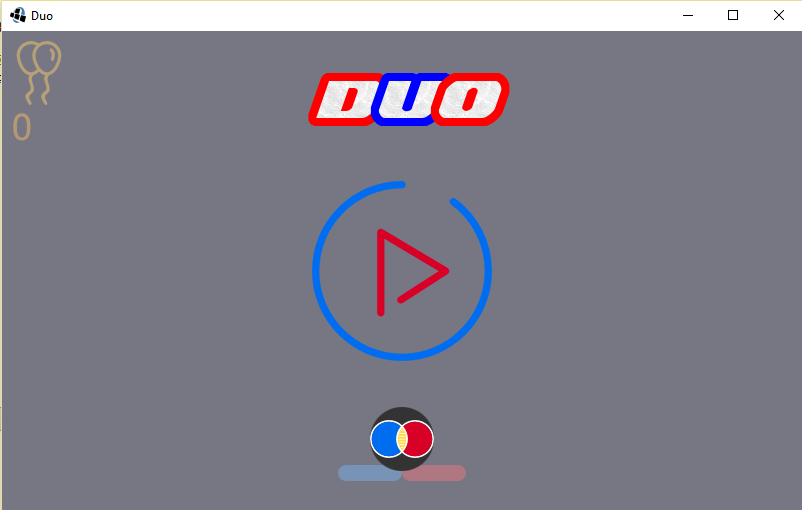
\includegraphics[width=0.7\linewidth]{screenshot011}
\end{center}

\newline \newline
Game screen ce include bombs, la fel si bonuses
\begin{center}
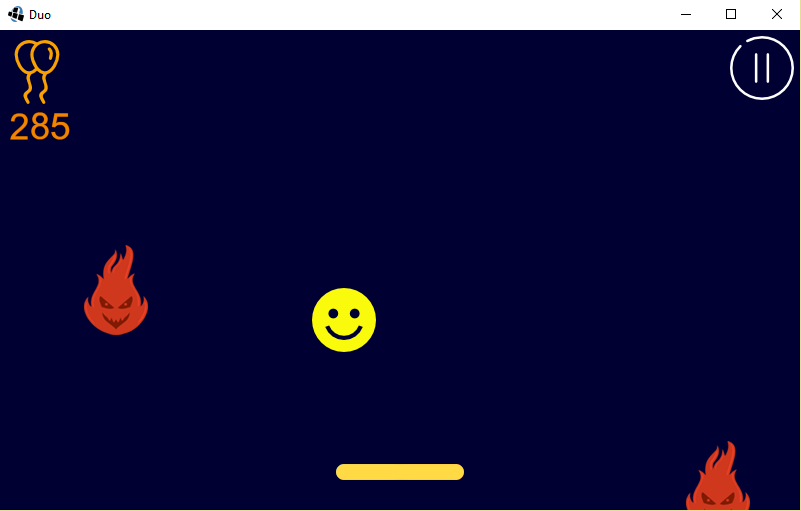
\includegraphics[width=0.6\linewidth]{screenshot012}
\end{center}

\newline \newline
PauseMenu in cazul tastarii PauseButton sau onPause app
\begin{center}
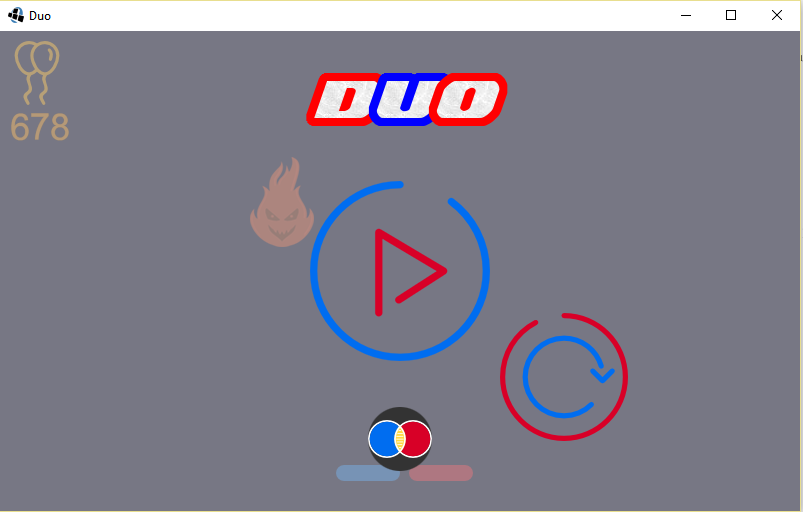
\includegraphics[width=0.7\linewidth]{screenshot013}
\end{center}

\newline \newline
Meniul in cazul GameOver la overlap-ul unui dintre atribute cu bombs:
\begin{center}
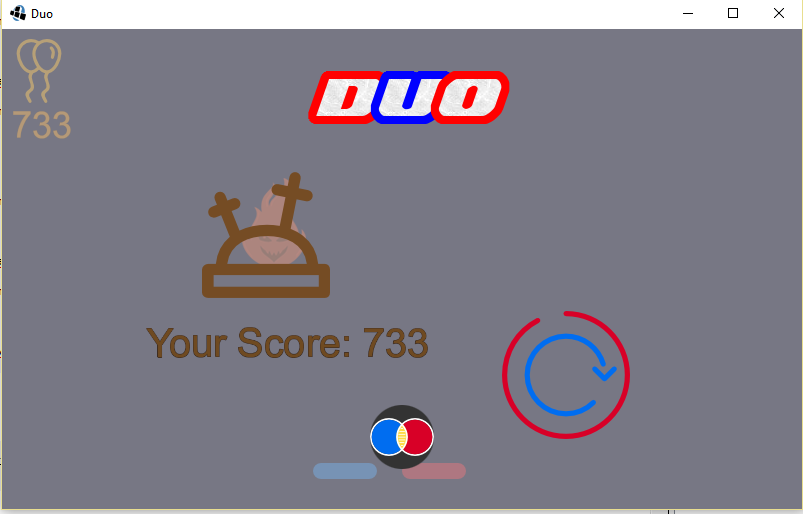
\includegraphics[width=0.7\linewidth]{screenshot014}
\end{center}
















\clearpage